% This must be in the first 5 lines to tell arXiv to use pdfLaTeX, which is strongly recommended.
\pdfoutput=1
% In particular, the hyperref package requires pdfLaTeX in order to break URLs across lines.

\documentclass[11pt]{article}

% Remove the "review" option to generate the final version.
\usepackage{acl}

% Standard package includes
\usepackage{times}
\usepackage{latexsym}

% For proper rendering and hyphenation of words containing Latin characters (including in bib files)
\usepackage[T1]{fontenc}
% For Vietnamese characters
% \usepackage[T5]{fontenc}
% See https://www.latex-project.org/help/documentation/encguide.pdf for other character sets

% This assumes your files are encoded as UTF8
\usepackage[utf8]{inputenc}

% This is not strictly necessary, and may be commented out,
% but it will improve the layout of the manuscript,
% and will typically save some space.
\usepackage{microtype}

% If the title and author information does not fit in the area allocated, uncomment the following
%
%\setlength\titlebox{<dim>}
%
% and set <dim> to something 5cm or larger.

\usepackage{graphicx}
\usepackage{tabularx}
\usepackage{soul}
\usepackage{fontawesome}
\usepackage{multirow}
\usepackage{longtable}
\usepackage{scrextend}
\usepackage{booktabs}
\usepackage{fontawesome}

\usepackage{subfigure}
\usepackage[ruled, linesnumbered]{algorithm2e}
\usepackage{pifont}%


\usepackage{array}
\newcolumntype{L}[1]{>{\raggedright\let\newline\\\arraybackslash\hspace{0pt}}m{#1}}
\newcolumntype{C}[1]{>{\centering\let\newline\\\arraybackslash\hspace{0pt}}m{#1}}
\newcolumntype{R}[1]{>{\raggedleft\let\newline\\\arraybackslash\hspace{0pt}}m{#1}}



% \usepackage{polyglossia}
% \usepackage{fontspec}
% \usepackage{amsfonts}

% %\newfontfamily\DejaSans{DejaVu Sans}
% \setmainlanguage{english}
% \setotherlanguages{bengali}
% \newfontfamily\bengalifont{Noto Sans Bengali}[Script=Bengali]





\usepackage{epstopdf}
\usepackage[utf8]{inputenc}

\usepackage{hyperref}
\usepackage{xstring}

\usepackage{color}

\title{M-BAD: A Multilabel Dataset for Detecting Aggressive Texts and Their Targets}

\author{Omar Sharif$^\mathbf{{\faPagelines}}$, Eftekhar Hossain{\textsuperscript{\faDollar}}\and Mohammed Moshiul Hoque$^\mathbf{{\faPagelines}}$\\
  {$^{\faPagelines}$}Department of Computer Science and Engineering \\
  \textsuperscript{{\faDollar}}Department of Electronics and Telecommunication Engineering\\
  {\textsuperscript{\faDollar}$^{\faPagelines}$}Chittagong University of Engineering \& Technology, Chattogram-4349, Bangladesh \\
         \texttt\{omar.sharif, eftekhar.hossain, moshiul\_240\}@cuet.ac.bd\\}


\begin{document}
\maketitle
\begin{abstract}
Recently, detection and categorization of undesired (e. g., aggressive, abusive, offensive, hate) content from online platforms has grabbed the attention of researchers because of its detrimental impact on society. Several attempts have been made to mitigate the usage and propagation of such content. However, most past studies were conducted primarily for English, where low-resource languages like Bengali remained out of the focus. Therefore, to facilitate research in this arena, this paper introduces a novel multilabel Bengali dataset (named \textit{\textbf{M-BAD}}) containing 15650 texts to detect aggressive texts and their targets. Each text of M-BAD went through rigorous two-level annotations. At the primary level, each text is labelled as either \textit{aggressive} or \textit{non-aggressive}. In the secondary level, the aggressive texts have been further annotated into five fine-grained target classes: \textit{religion}, \textit{politics}, \textit{verbal}, \textit{gender} and \textit{race}. Baseline experiments are carried out with different machine learning (ML), deep learning (DL) and transformer models, where Bangla-BERT acquired the highest weighted $f_1$-score in both detection (0.92) and target identification (0.83) tasks. Error analysis of the models exhibits the difficulty to identify context-dependent aggression, and this work argues that further research is required to address these issues.
\end{abstract}

\section{Introduction}
Social media platforms have become a powerful tool to spontaneously connect people and share information with effortless access to the internet. These platforms provide users with a cloak of anonymity that allows them to speak their opinions publicly. Unfortunately, this power of anonymity is misused to disseminate aggressive, abusive, hatred and illegal content. In the recent past, these mediums have been used to incite religious, political and communal violence \cite{hartung-etal-2017-ranking}. A significant portion of such incidents has been communicated through textual content \cite{trac-2020-trolling,nlp4if-2021-nlp}. Therefore, it has become crucial to develop automated systems to restrain the proliferation of such undesired or aggressive texts. This issue has been taken seriously in English, German, and other high-resource languages \cite{caselli-etal-2021-hatebert,aksenov-etal-2021-fine}. However, minimal research effort has been made in low-resource languages, including Bengali. Systems developed in English or other languages can not detect detrimental texts written in Bengali due to the significant variations in language constructs and morphological features. Nevertheless, people use their regional language to communicate over social media. Therefore, developing benchmark datasets and regional language tools is monumental to tackle the undesired text detection challenges. This work develops  M-BAD containing 15650 texts using a two-level hierarchical annotation schema. In level-1, texts are categorized into binary classes: aggressive or non-aggressive. In level-2, 8289 aggressive texts are further annotated with multilabel targets. These labels are used to identify aggression's target into five fine-grained classes, such as \textit{religion}, \textit{gendered}, \textit{race}, \textit{verbal} and \textit{politics} (detailed taxonomy discussed in Section \ref{section3}). Proper annotation guidelines and the detailed statistics of the dataset is described to ensure M-BAD's quality. Several experiments are performed using ML, DL and transformer models to assess the task. The experiments demonstrate that (i) transformer models are more effective in detecting aggressive texts and their targets than ML/DL counterparts, (ii) covert propagation of aggression using ambiguous, context-dependent and sarcastic words is difficult to identify. The significant contributions of this work can be summarized as follows,

\begin{itemize}
     \item Study two new problems from the perspective of low-resource language (i.e. Bengali), \textit{(i)} detecting aggressive texts and \textit{(ii)} identifying the multilabel targets of aggression. 
    \item Release a new benchmark aggressive dataset labelled with the target of aggression and detailed annotation steps. 
    \item Perform baseline experimentation on the developed dataset (M-BAD) to benchmark the two problems, providing the first insight into this challenging task.
\end{itemize}

\textbf{Reproducibility:} The resources to reproduce the results are available at \textcolor{blue}{\href{https://github.com/omar-sharif03/M-BAD}{https://github.com/omar-sharif03/M-BAD}}. The appendix contains details about data sources, annotators and a few samples of M-BAD.

\section{Related Work}
This section briefly describes the past studies related to aggression and other undesired content detection concerning non-Bengali and Bengali languages. 

\textbf{Non-Bengali aggressive text classification:}
\citet{kumar-etal-2018-benchmarking} compiled a dataset of 15000 aggression annotated comments in English and Hindi with three classes: \textit{overtly aggressive, covertly aggressive, non-aggressive}. In their subsequent work \citep{kumar-etal-2020-evaluating}, Bengali aggressive comments were added in the corpus. Early works with neural network techniques such as LSTM \citep{nikhil-etal-2018-lstms}, CNN \citep{kumari-singh-2020-ai}, combination of shallow and deep network \citep{golem-etal-2018-combining} achieved good accuracy. However, with the arrival of BERT based models, it acquired superior performance and outperformed all the models on these datasets \citep{risch-krestel-2020-bagging,gordeev-lykova-2020-bert,
sharif-etal-2021-nlp}. \citet{bhardwaj2020hostility} developed a multilabel dataset in Hindi with five hostile classes: \textit{fake, defamation, offensive, hate, non-hostile}. Their baseline system was implemented with m-BERT embedding and SVM. \citet{leite-etal-2020-toxic} introduced a multilabel toxic language dataset. The dataset contains 21k tweets manually annotated into seven categories: \textit{insult}, \textit{LGBTQ+phobia}, \textit{obscene}, \textit{misogyny}, \textit{racism}, \textit{non-toxic} and \textit{xenophobia}. They also performed baseline evaluation with the variation of BERT models. In a similar work, \citet{moon-etal-2020-beep} developed a corpus to detect toxic speech in Korean online news comments. 

\textbf{Bengali aggressive text classification:} No significant research has been conducted yet to detect multilabel aggression in Bengali. The scarcity of benchmark corpora is the primary reason behind this. Few works have been conducted to develop datasets and models in other correlated domains such as hate, abuse, fake and offence. \citet{karim2021deephateexplainer} developed a hate speech dataset of 3000 samples with four categories: \textit{political}, \textit{personal}, \textit{religious}, \textit{geopolitical}. \citet{8843606} presented a dataset comprised of 4.7k abusive Bengali texts collected from online platforms. They proposed LSTM based classifier to categorize texts into seven classes. However, they did not investigate other DL models' performance, which might get similar accuracy with less computational cost. To detect the threat and abusive language, a dataset of 5.6k Bengali comments is created by \citet{8934609}. In recent work, \citet{sharif2021constraint} introduced a benchmark Bengali aggressive text dataset. They employed a hierarchical annotation schema to divide the dataset into two coarse-grained (aggressive, non-aggressive) and four fine-grained (political, religious, verbal, gendered) aggression classes. In their later work \cite{SHARIF2021}, they extended the dataset from 7.5k texts to 14k texts.

\textbf{Differences with existing studies:} As far as we are concerned, very few works have been accomplished to detect aggressive texts and identify the target of aggression (e.g. religion, gender, race). Existing works \cite{SHARIF2021,zampieri-etal-2019-predicting,kumar-etal-2018-aggression} have framed it as a multi-class classification problem and ignored the overlapping phenomena of classes. However, a text can express aggression towards multiple targets simultaneously. Suppose a text has an aggressive write up against political women, expressing political and gendered aggressions. The proposed work addresses the issues that are previously overlooked and differs from the existing research in the following ways, (i) develop a novel Bengali aggressive text dataset annotated with the multiple targets of an aggressive text. As our knowledge goes, this is the first attempt to develop such a dataset in Bengali, (ii) illustrate a detailed annotation guideline which can be followed to develop resources for the similar domains in Bengali and other low-resource languages, (iii) perform experimentation with multilabel classes with various ML, DL and transformer-based models.


\section{Dataset Development Taxonomy}
\label{section3}
 This work presents a two-level hierarchical annotation schema to develop a novel multilabel aggression dataset in Bengali (M-BAD). Level-1 has two coarse-grained categories: aggressive and non-aggressive. In contrast, level-2 has five fine-grained multilabel target classes (religion, politics, verbal, gender, race). This work differs from previous work done by \citet{SHARIF2021} in two ways; (i) overlapping phenomena between aggression targets are considered, (ii) a new target class (i.e., racial aggression) is added into the M-BAD. Figure 1 illustrates the taxonomic structure of M-BAD.

\begin{figure}[h!]
\centering
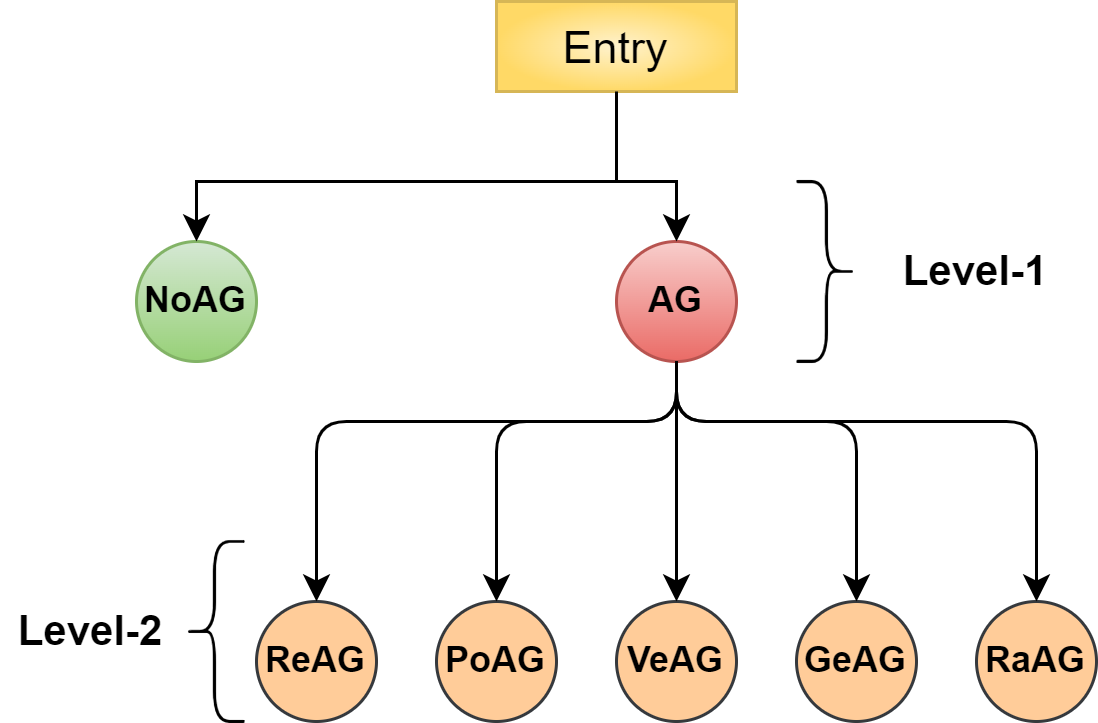
\includegraphics[width =\linewidth]{Figure/taxonomy.png}
\caption{Taxonomic structure} 
\label{hist}
\end{figure}

Because of the subjective nature of the dataset, it is crucial to have a clear understanding of the categories. It helps develop a quality dataset by mitigating annotation biases and reducing ambiguities. After analyzing past studies \cite{SHARIF2021,bhardwaj2020hostility,zampieri-etal-2019-predicting,vidgen-etal-2021-introducing} on textual aggression and other related phenomena, we differentiate between the coarse-grained and fine-grained categories.

%\subsection{Coarse-grained Aggression Classes}
\paragraph{Coarse-grained Aggression Classes}: The system initially identifies an input text as aggressive (AG) or non-aggressive (NoAG) classes.
\begin{itemize}
    \item \textbf{(AG)}: excite, attack or seek harm to the individual, group or community based on a few criteria such as gender identity, political ideology, sexual orientation, religious belief, race, ethnicity and nationality.
    \item \textbf{(NoAG)}: do not contain any aggressive statements or express any evil intention to harm others. 
\end{itemize}

\paragraph{Fine-grained Target Classes:} An AG text is further classified into five fine-grained categories: religious aggression (ReAG), political aggression (PoAG), verbal aggression (VeAG), gendered aggression (GeAG) and racial aggression (RaAG). Each of the classes is defined in the following:
\begin{itemize}
\item \textbf{ReAG}: excite violence by attacking religion, religious organization or religious belief (Catholic, Hindu, Jew, or Islam, etc.) of a community 
    \item \textbf{PoAG}: demean political ideology, provoke followers of political parties, or incite people in against law enforcement agencies and state. 
    \item \textbf{VeAG}: seek to do evil or harm others, denounce the social status by using curse words, obscene words, outrageous and other threatening languages. 
    \item  \textbf{GeAG}: attack an individual or group by making aggressive reference to sexual orientation, sexuality, body parts, or other lewd contents.
    \item \textbf{RaAG}: insult or attack some and promote aggression based on race. 
\end{itemize}

\section{M-BAD: Multilabel Aggression Dataset}
As far as we are concerned, no dataset is available to date for detecting or classifying multilabel aggressive texts and their targets in Bengali. However, the availability of a benchmark dataset is the prerequisite to developing any deep learning-based intelligent text classification system. This drawback motivates us to construct \textbf{M-BAD}: a novel multilabel Bengali aggressive text dataset. This work follows the guidelines and directions given by \cite{SHARIF2021,vidgen2020directions} to ensure the quality of the dataset. This section briefly describes the data collection and annotation steps with detailed statistics of M-BAD. 

\subsection{Data Collection}
We have manually accumulated {\textbf{16000}} aggressive and non-aggressive texts from different social platforms within the duration from 16 June to 27 December 2021. During this period, we only collected those texts that were posted, composed or shared after 1 January 2020. Potential texts were accumulated from YouTube channels and Facebook pages affiliated with political organizations, religion, newsgroups, artists, authors, celebrities, etc. Appendix \ref{source} presents detailed statistics of the data collection sources.

Aggressive texts were cumulated from comments and posts that express aggression or excite violence. User profiles were also scanned who promoted, shared, or glorified aggression information to acquire additional texts. On the other hand, non-aggressive posts have been collected from news/comments/posts related to sports, education, entertainment, science and technology. Furthermore, while collecting aggressive texts, many data samples were found that did not express any aggression. Such texts were added to the corpus. We did not store any personal information (name, phone number, birth date, location) of the users during data accumulation. Each sample text is anonymized in the dataset. Thus, we do not know who has posted or created the collected texts. Finally, a few preprocessing filters are applied to remove inappropriate texts. 255 samples are discarded based on the following filtering criteria, (i) contains non-Bengali texts, (ii) has length fewer than three words, (iii) duplication. Remaining {\textbf{15745}} texts passed to the annotators for manual labelling. 

\subsection{Annotation Process}
Section \ref{section3} describes the annotation schema and class definitions used to annotate the texts. Six annotators carried the annotation: four undergraduate and two graduate students. An expert verified the label in case of disagreement. Appendix \ref{anno-demo} illustrates the detailed demographics of annotators. Annotators were split into three groups (two in each), and each group labelled a different subset of processed texts. To achieve quality annotations, we trained the annotators to define classes and associated examples. We tried to ensure that annotators understood what an aggressive text is and how to determine the target of aggression. Moreover, annotators are carefully guided in the weekly lab meetings. 

Two annotators annotated each text, and the final label was assigned based on the agreement between the annotators. In case of disagreement, an expert resolve the issue through deliberations with the annotators. During the final label assignment, we found {95} texts that did not fall into any defined aggression categories and subsequently discarded them. Finally, we get M-BAD, an aggression dataset annotated with their targets containing \textbf{15650} texts. Appendix \ref{sample} shows few samples of M-BAD.  

\begin{table}[h!]
\begin{center}
% \begin{tabular}{L{1.8cm} L{1.2cm}C{1.5cm}C{1.2cm}}
\small
\begin{tabular}{llcc}
\hline
 &  & \textbf{$\kappa$-score}  & \textbf{Average}\\
\hline
\multirow{2}{*}{Level-1}& AG & 0.85 &\multirow{2}{*}{0.77} \\
& NoAG & 0.69 & \\
\hline
\multirow{5}{*}{Level-2}& ReAG & 0.55  & \multirow{5}{*}{0.62} \\
& PoAG & 0.61 &    \\
& VeAG & 0.62 &      \\
& GeAG  & 0.67 &    \\
& RaAG & 0.65 & \\
\hline 
 
\end{tabular}
\caption{Kappa ($\kappa$) score on each annotation level}
\label{kappa-score}
\end{center}
\end{table}
We measure the inter-annotator agreement using kappa score \cite{cohen} to check the validity of annotations. Table \ref{kappa-score} presents the \textit{$\kappa$-score} on both coarse-grained and fine-grained classes. The table shows that agreement is higher (0.77) in coarse-grained classes. The agreement is consistently `moderate' ($\approx0.62$) among the fine-grained classes but a bit lower in ReAG. Scores indicate difficulty in detecting targets of aggression by the annotators. Analysis reveals that sarcastic, implicit and ambiguous words made this difficult.


\subsection{Dataset Statistics}
For training and evaluation purposes, the developed M-BAD is divided into the train (80\%), test (10\%), and validation (10\%) split using a stratified strategy. The identical split ratio is used for both coarse-grained and multilabel fine-grained experiments. Table \ref{dataset-split} presents the class-wise distribution of the texts for both Level-1 and Level-2. It is noticed that the distributions are slightly imbalanced with Level-2, which will be very challenging to handle in a multilabel setup.

\begin{table}[h!]
\begin{center}
\small
%\begin{tabular}{L{1.3cm}C{1cm}C{1cm}C{1cm}C{1cm}}
\begin{tabular}{lcccc}
\hline
 \textbf{Class}  & \textbf{Train} & \textbf{Test} & \textbf{Valid} & \textbf{Total} \\
 \hline 
 ReAG  & 2391 & 327 & 305 & 3023 \\
 PoAG & 2408 & 310 & 275 & 2993\\
 VeAG & 3939 & 498 &  472 & 4909\\
 GeAG & 1306 & 148 &  167 & 1621\\
 RaAG & 175 & 21 &  28 & 224\\
 \hline
 NoAG & 5893 & 710 & 758 & 7361\\
 AG & 6642 & 840 & 807 & 8289\\
 \hline
\end{tabular}
\caption{Number of instances in train, test and validation sets for each category}
\label{dataset-split}
\end{center}
\end{table}

% \begin{table*}[h!]
% \begin{center}
% % \begin{tabular}{L{1.8cm} L{1.2cm}C{1.5cm}C{1.2cm}}
% \small
% \begin{tabular}{lcc|ccccc}


% & \multicolumn{2}{c}{\textbf{Level-1}} & \multicolumn{5}{c}{\textbf{Level-2}}\\
% \hline
%  & \textbf{AG} & \textbf{NoAG} & \textbf{ReAG} & \textbf{PoAG}  & \textbf{VeAG} & \textbf{GeAG} & \textbf{RaAG}\\
% \hline
% \#Words & 80553 & 106573 & 30748 & 28410 & 42342  & 13817 &  1711 \\
% \#Unique words & 17413 & 24617 & 9093 & 8496  & 11587  & 4796 &  1026 \\
% Max. text length & 141 & 387 & 75 & 92 & 69  & 69 & 53    \\
% Avg. \#words/text & 14.76 & 17.95 & 12.76  & 12.02  & 10.79  & 10.53 & 10.00  \\
%  \hline 
% \end{tabular}
% \caption{Training set statistics.}
% \label{data-summary}
% \end{center}
% \end{table*}


\begin{table}[h!]
\begin{center}
% \begin{tabular}{L{1.8cm} L{1.2cm}C{1.5cm}C{1.2cm}}
\small
\begin{tabular}{ll|cC{1.2cm}C{1.5cm}}

\hline
& \textbf{Class}& \textbf{\#Words} & \textbf{\#Unique words}  & \textbf{Avg. \#words/text} \\ 
\hline

\multirow{2}{*}{Level-1} & AG & 80553 & 17413 &12.12\\
& NoAG & 106573 & 24617  & 18.08 \\
\hline

\multirow{5}{*}{Level-2} & ReAG & 30748 & 9093 & 12.85 \\
& PoAG & 28410 & 8496  & 11.79\\
& VeAG & 42342 & 11587  & 10.74 \\
& GeAG & 13817 & 4796  & 10.57\\
& RaAG & 1711 & 1206 & 9.77\\
 \hline 
\end{tabular}
\caption{Training set statistics in each level and class}
\label{data-summary}
\end{center}
\end{table}

To obtain in-depth insights, training set is further analyzed which is reported in Table \ref{data-summary}. The statistics illustrated that in Level-1, NoAG class has the highest number of words ($\approx$106k) and unique words ($\approx$24k) compared to the AG class. Meanwhile, in Level-2, VeAG has the maximum number of words ($\approx$42k) and unique words ($\approx$11k) while RaAG class has the lowest ($\approx$1.7k, $\approx$1.2k). However, the average number of words per text ranges from 10 to 12 among the aggression categories. Figure \ref{hist} shows the histogram of the texts length of each category. It is observed that $\approx$5000 texts of NoAG class have a length between $\approx$15-40. On the other hand, most of the length of the texts falls between 5-30 in VeAG class while $\approx$ 1000 texts of RaAG class has a length $<20$. It is also noticed that only a small number of texts have length $>50$. 
\begin{figure}[h!]
\centering
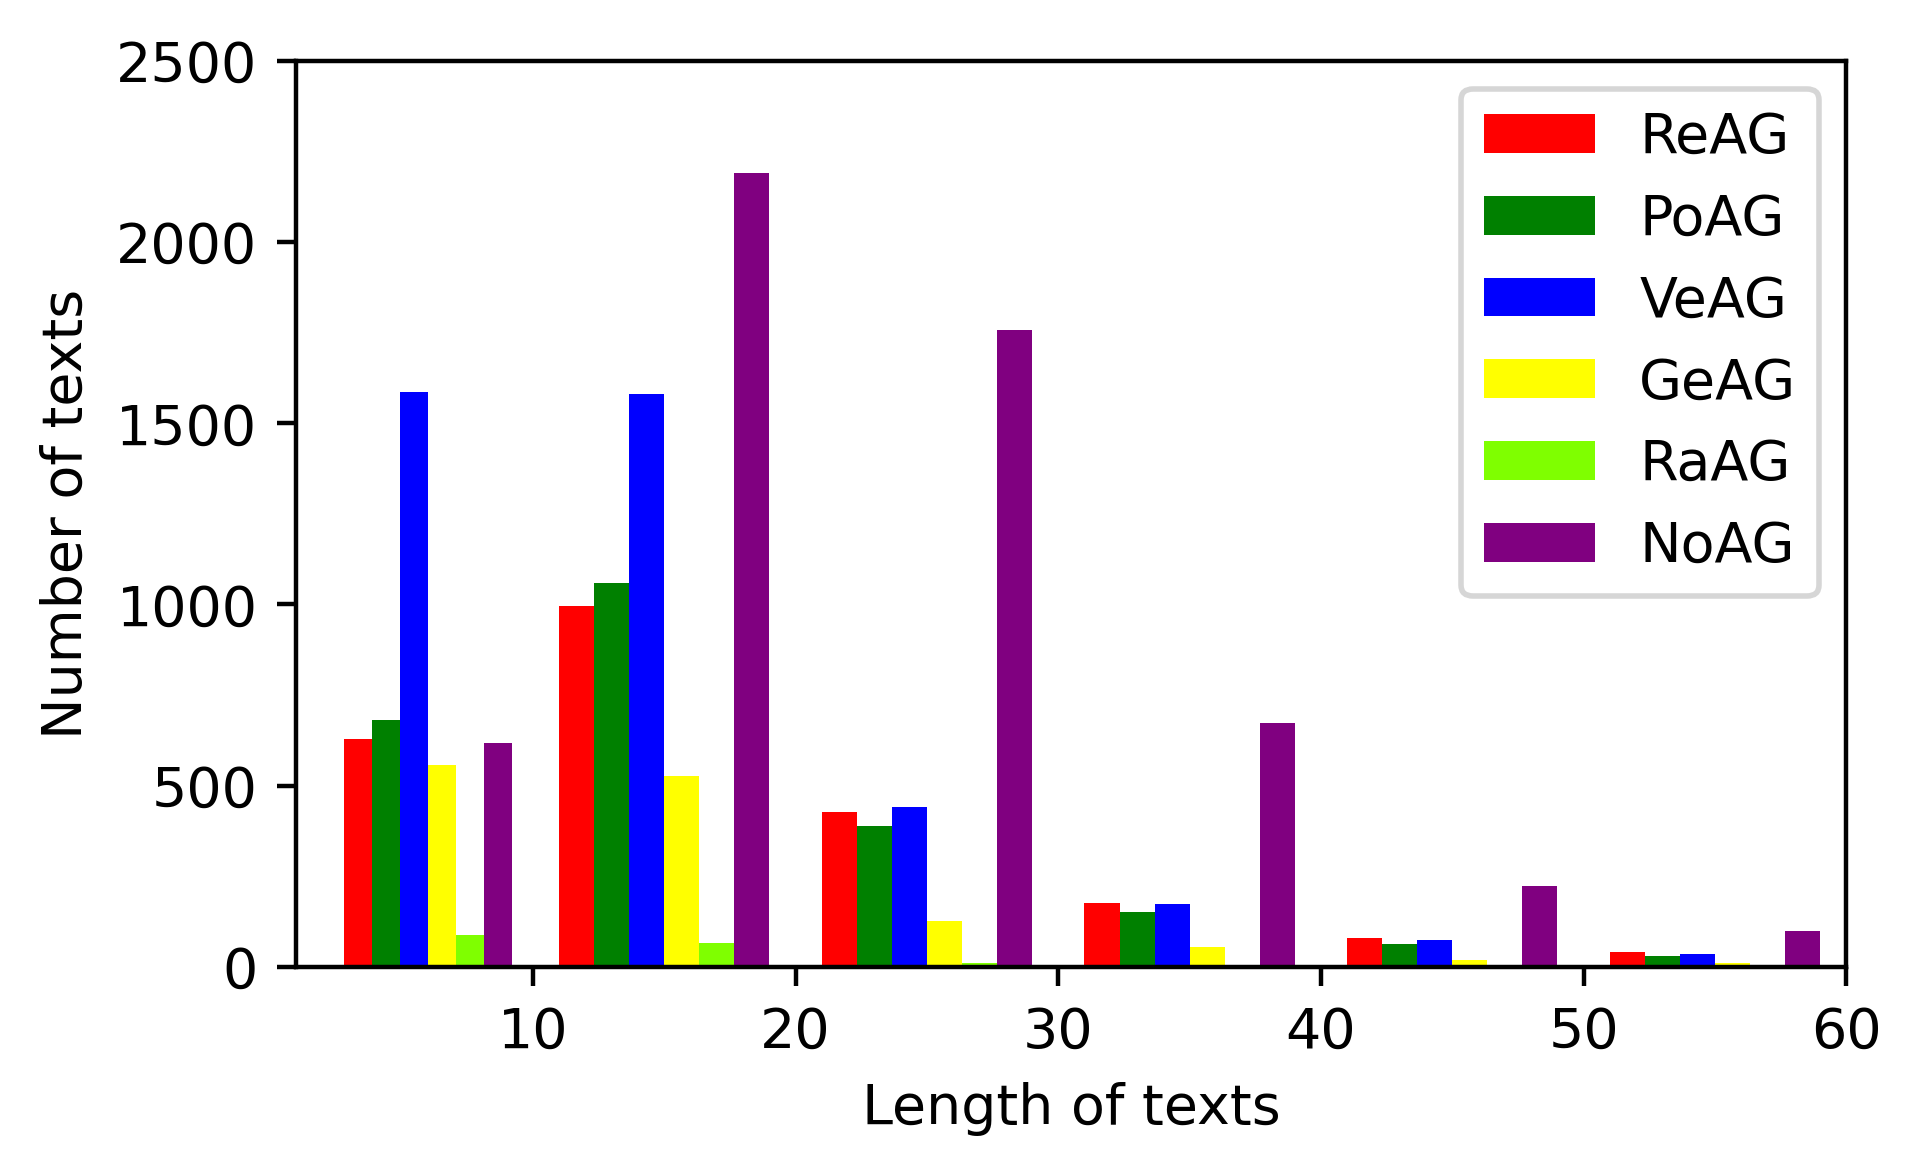
\includegraphics[width =\linewidth]{Figure/dist.png}
\caption{Histogram of the text length for each categories} 
\label{hist}
\end{figure}

\begin{table}[h!]

\begin{center}
% \begin{tabular}{L{1.8cm} L{1.2cm}C{1.5cm}C{1.2cm}}
\small
\begin{tabular}{lcccc}
\hline
  & \textbf{PoAG}  & \textbf{VeAG} & \textbf{GeAG} & \textbf{RaAG}  \\
\hline
ReAG   & 0.38  &  0.47 & 0.36 & 0.18 \\
PoAG   &  & 0.42 & 0.29 & 0.16  \\
VeAG   &  & & 0.50 & 0.25   \\
GeAG   &  & & & 0.23  \\
\hline
& \textbf{NoAG}& & &  \\
\hline
AG  &0.22 & & & \\

 \hline 
\end{tabular}
\caption{Jaccard similarity of 400 most frequent words between each pair of classes}
\label{jaccard}
\end{center}
\end{table}

We calculated the Jaccard similarity scores between the most 400 frequent words for quantitative analysis. Table \ref{jaccard} presents the similarity values among each pair of categories from Level-1 and Level-2. The VeAG-GeAG pair obtained the highest similarity score (0.50), while the PoAG-RaAG pair got the lowest score (0.16). It is observed that VeAG class has maximum similarity with almost all the classes except RaAG.

\section{Methodology}
Several computational models are investigated to develop the target aware aggression identification system. At first, the investigation is carried out for classifying the aggressive texts, and then we develop models for categorizing the target of the aggression (ReAG, PoAG, VeAG, GeAG, RaAG) considering the multilabel scenario. Machine learning and deep learning-based methods are employed to build the system. This section briefly discussed the techniques and methods used to develop the system. 

% \subsection{Data Preprocessing}
% The raw text contains various inconsistencies such as flawed characters (i.e !@\$\%\&) punctuation’s, symbols, special characters, and emoticons. In the preprocessing phase, all of these are dispelled from the texts. Besides, we also excluded the Bengali stopwords (i.e., conjunction, pronoun, preposition etc.) from the texts. 

\subsection{ML-based methods}
Two ML-based methods, Logistic Regression (LR) \cite{sharif2019automatic} and Naive Bayes with Support Vector Machine (NBSVM) \cite{wang2012baselines} have been investigated for the classification task. Bag of words (BoW) features are used to train these models. The LR model is built with the `lbfgs' optimizer and `l2' regularization technique. Apart from this, the inverse regularization parameter $C$ settled to $1.0$. On the other hand, for NBSVM, the additive smoothing ($\alpha$) and regularization parameters ($C$) are settled at $1.0$ whereas the interpolation value is selected to $\beta$ = $0.25$.

\subsection{DL-based Methods}
Several popular DL methods are also investigated including BiGRU \cite{marpaung2021hate} and pretrained transformers \cite{vaswani2017attention} to identify the multi-label textual aggression.  
\paragraph{BiGRU+FastText:} The FastText \cite{joulin2016fasttext} embeddings are used as the input of the BiGRU model. Before that, a 1D spatial dropout technique is applied over the embedding features and then fed to a BiGRU layer with 80 hidden units. The last time step hidden output from the BiGRU is passed to a 1D global average pooling and a 1D global max-pooling layer. Subsequently, the two pooling layers outputs are concatenated and propagated to the classification layer.    
\paragraph{Pretrained Transformers:} In recent years, transformer \cite{vaswani2017attention} models trained on multilingual and monolingual settings achieved outstanding result in solving undesired text classification related tasks \cite{SHARIF2021,hossain-etal-2021-nlp}. As our task deals with a dataset of low-resource language, we employed three transformer-based models: (i) Multilingual Bidirectional Encoder Representations for transformers (m-BERT) \cite{mbert} (ii) BERT for Bangla language (Bangla-BERT) \cite{banglabert}, and (iii) BERT for Indian languages (Indic-BERT) \cite{indicbert}. The models have culled from the hugging face\footnote{https://huggingface.co/} transformers library and fine-tuned them with default arguments on the developed dataset.  

Both ML and DL-based models are trained for two classification tasks: coarse-grained and multilabel fine-grained. To allow the reproducibility of the models and mitigate the training complexity, we use identical hyperparameters values for both classification tasks. We employed the Ktrain \cite{maiya2020ktrain} wrapper that provides easy training and implementation of the models. For multilabel classification, we enabled the Ktrain default multilabel settings. The BiGRU+FastText model is trained with a learning rate of $7e^{-3}$ while the transformer models with $8e^{-5}$. The models are trained using the triangular policy method \cite{smith2017cyclical} for $20$ epochs with a batch size of 32. To save the best intermediate models, we utilized the early stopping criterion. 

\section{Experiments}
The experiments were carried out in a google collaboratory platform with a GPU environment. The evaluation of the dataset is performed based on the weighted $f_1$-score. Due to the highly skewed distribution of the classes, we considered macro $f_1$-score (MF1) as our primary metric in multilabel evaluation. Besides, the individual class performance is measured through precision (P), recall (R), and $f_1$-score (F1) matrices.  

% In case of coarse grained experiment, all the aggression categories are considered as one single aggression class and then perform the binary (Aggression/Not-Aggression) classification.     

\subsection{Results}
Table \ref{cg}  presents the outcome of the different models on the test set concerning the coarse-grained classification. In terms of weighted $f_1$-score (WF1), both LR and NBSVM obtained an identical score of $0.91$ while BiGRU + FastText and m-BERT model got a slightly low score ($0.90$). However, the Bangla-BERT model achieved the highest F1 across the two coarse-grained classes (AG/NoAG = $0.92$) and thus outperformed all the models by achieving the highest WF1 score of $0.92$. 

\begin{table}[h!]
\centering
\scriptsize
\begin{tabular}{cccc|ccc|c}

 & \multicolumn{3}{c}{\textbf{AG}}& \multicolumn{3}{c}{\textbf{NoAG}}\\
\hline
Method &\textbf{P}&\textbf{R}&\textbf{F1}&\textbf{P}&\textbf{R}&\textbf{F1}&\textbf{WF1}\\
\hline
LR & 0.93 & 0.90 & 0.91 & 0.89 & 0.92 & 0.91 & 0.91  \\

NBSVM & 0.94 & 0.89 & 0.91 & 0.89 & 0.94 & 0.91 & 0.91 \\

BG+FT &  0.88 & 0.93 & 0.90 & 0.92 & 0.87 & 0.89 & 0.90  \\

m-BERT & 0.90 & 0.89 & 0.90 & 0.89 & 0.90 & 0.89 & 0.90 \\

Indic-BERT & 0.88 & 0.90 & 0.89 & 0.89 & 0.87 & 0.88 & 0.89  \\

Bangla-BERT &  0.93 & 0.91 & 0.92 & 0.91 & 0.93 & 0.92 & \textbf{0.92} \\
\hline            
\end{tabular}
\caption{\label{cg}{Performance of the Coarse-grained classification on the test set. Here, BG+FT represents BiGRU+FastText model}}
\end{table}

Table \ref{fg} reports the evaluation results of the multilabel fine-grained classification. The outcome illustrates that the NBSVM obtained the lowest MF1 (0.61) and WF1 score (0.77). Both Indic-BERT and BiGRU+FastText models acquired identical WF1 of 0.79. Meanwhile, macro and weighted $f_1$-score is slightly (MF1 $\approx$4\%, WF1 $\approx$ 1\%) improved with the m-BERT model. However, the Bangla-BERT model exceeds all the models by achieving the highest MF1 (0.72) and WF1 (0.83). In terms of class-wise performance, Bangla-BERT obtained the highest $f_1$-score in four fine-grained aggression classes: ReAG (0.94), PoAG (0.92), VeAG (0.81), and GeAG (0.68). One interesting finding is that in RaAG class, some models (LR, NBSVM, Indic-BERT) did not identify a single instance correctly. Moreover, the models' performance degrades with the classes (GeAG, RaAG) having fewer training samples than other classes. Thus, a large dataset with balanced data distribution needs to be developed for classifying the problematic multilabel samples. 

\begin{table*}[h!]
\centering
\renewcommand*{\arraystretch}{1.1}
\scriptsize
\begin{tabular}{cccc|ccc|ccc|ccc|ccc|cc}

 & \multicolumn{3}{c}{\textbf{ReAG}}& \multicolumn{3}{c}{\textbf{PoAG}}& \multicolumn{3}{c}{\textbf{VeAG}} & \multicolumn{3}{c}{\textbf{GeAG}} & \multicolumn{3}{c}{\textbf{Racism}} \\
\hline
Method &\textbf{P}&\textbf{R}&\textbf{F1}&\textbf{P}&\textbf{R}&\textbf{F1}&\textbf{P}&\textbf{R}&\textbf{F1}&\textbf{P}&\textbf{R}&\textbf{F1}&\textbf{P}&\textbf{R}&\textbf{F1}&\textbf{MF1}&\textbf{WF1}\\
\hline
LR & 0.93 & 0.84& 0.88 & 0.93 & 0.81 & 0.86 &  0.74 & 0.75 & 0.75 & 0.75 & 0.51 & 0.61 & 0.00 & 0.00 & 0.00 & 0.66 & 0.77  \\

NBSVM & 0.93 & 0.85 & 0.89 & 0.95 & 0.82 & 0.88 & 0.74 & 0.73 & 0.74 & 0.72 & 0.47 & 0.57 & 0.00 & 0.00 & 0.00 & 0.61 & 0.77   \\

BG+FT & 0.89 & 0.89 & 0.89 & 0.90 & 0.85 & 0.87 & 0.75 & 0.74 & 0.75 & 0.67 & 0.64 & 0.66 & 0.50 & 0.11 & 0.18 & 0.67 & 0.79   \\

m-BERT & 0.92 & 0.89 & 0.90 & 0.90 & 0.93 & 0.92 & 0.81 & 0.71 & 0.76 & 0.71 & 0.60 & 0.65 & 0.50 & 0.25 & 0.33 & 0.71 & 0.80 \\

Indic-BERT &  0.89 & 0.90 & 0.89 & 0.94 & 0.87 & 0.90 & 0.75 & 0.75 & 0.75 & 0.68 & 0.64 & 0.66 & 0.00 & 0.00 &      0.00 & 0.64 & 0.79  \\

Bangla-BERT &  0.94 & 0.93 & 0.94 & 0.93 & 0.92 & 0.92 & 0.79 & 0.82 & 0.81 & 0.70 & 0.66    & 0.68 & 0.67 & 0.14 & 0.24 & \textbf{0.72} & \textbf{0.83}  \\

\hline            
\end{tabular}
\caption{\label{fg}{Fine-grained classification performance on the test set. Here, MF1 indicates the macro $f_1$-score}
}
\end{table*}


\begin{figure*}[h!]
  \centering
  \subfigure[NoAG]{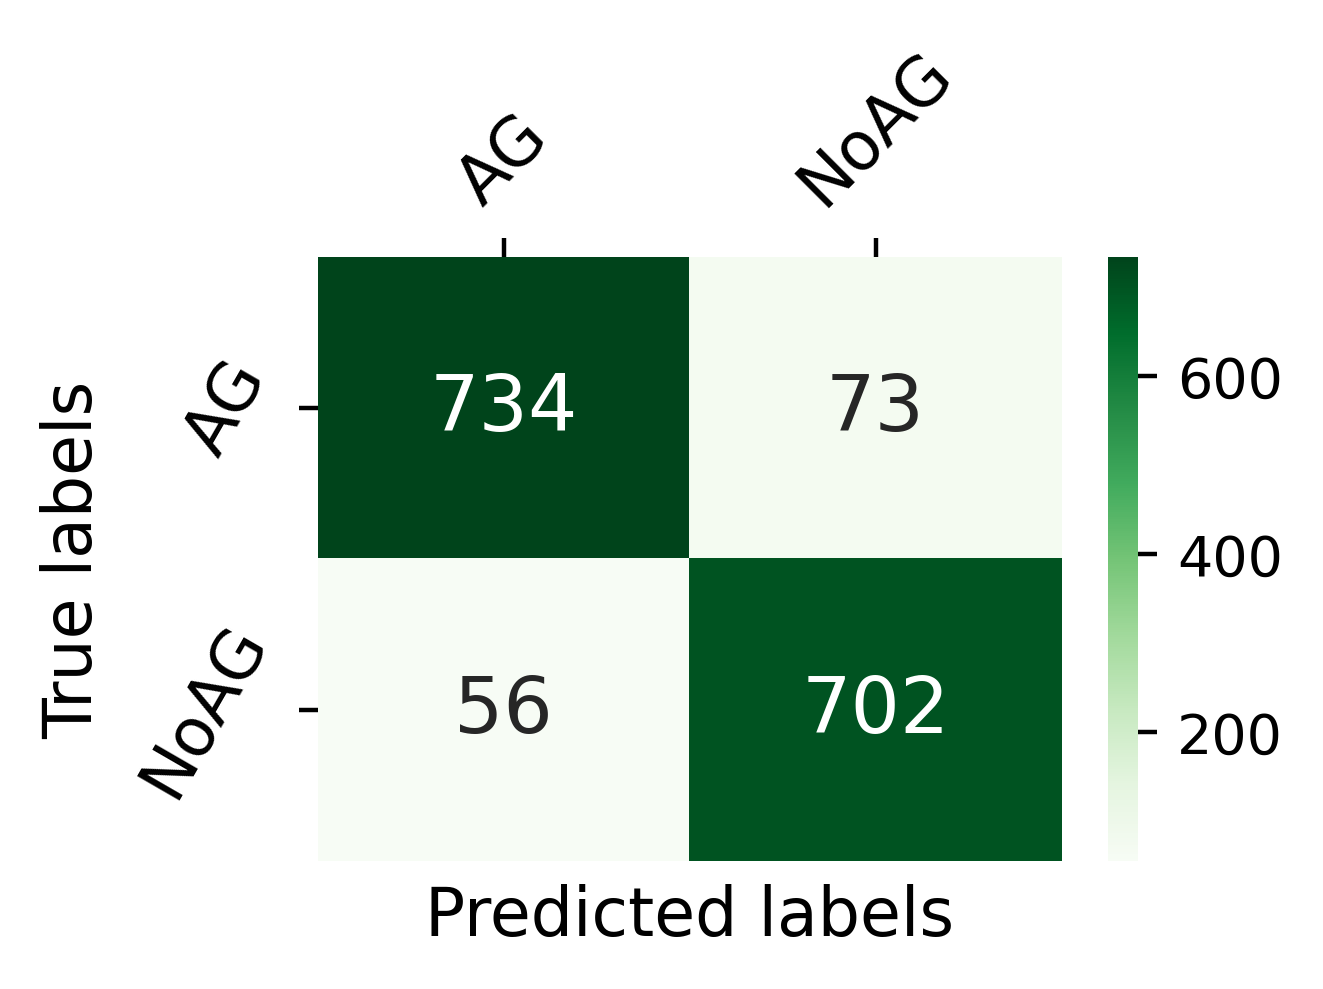
\includegraphics[width= 0.3\textwidth]{Figure/NoAG.png}}
  \subfigure[ReAG]{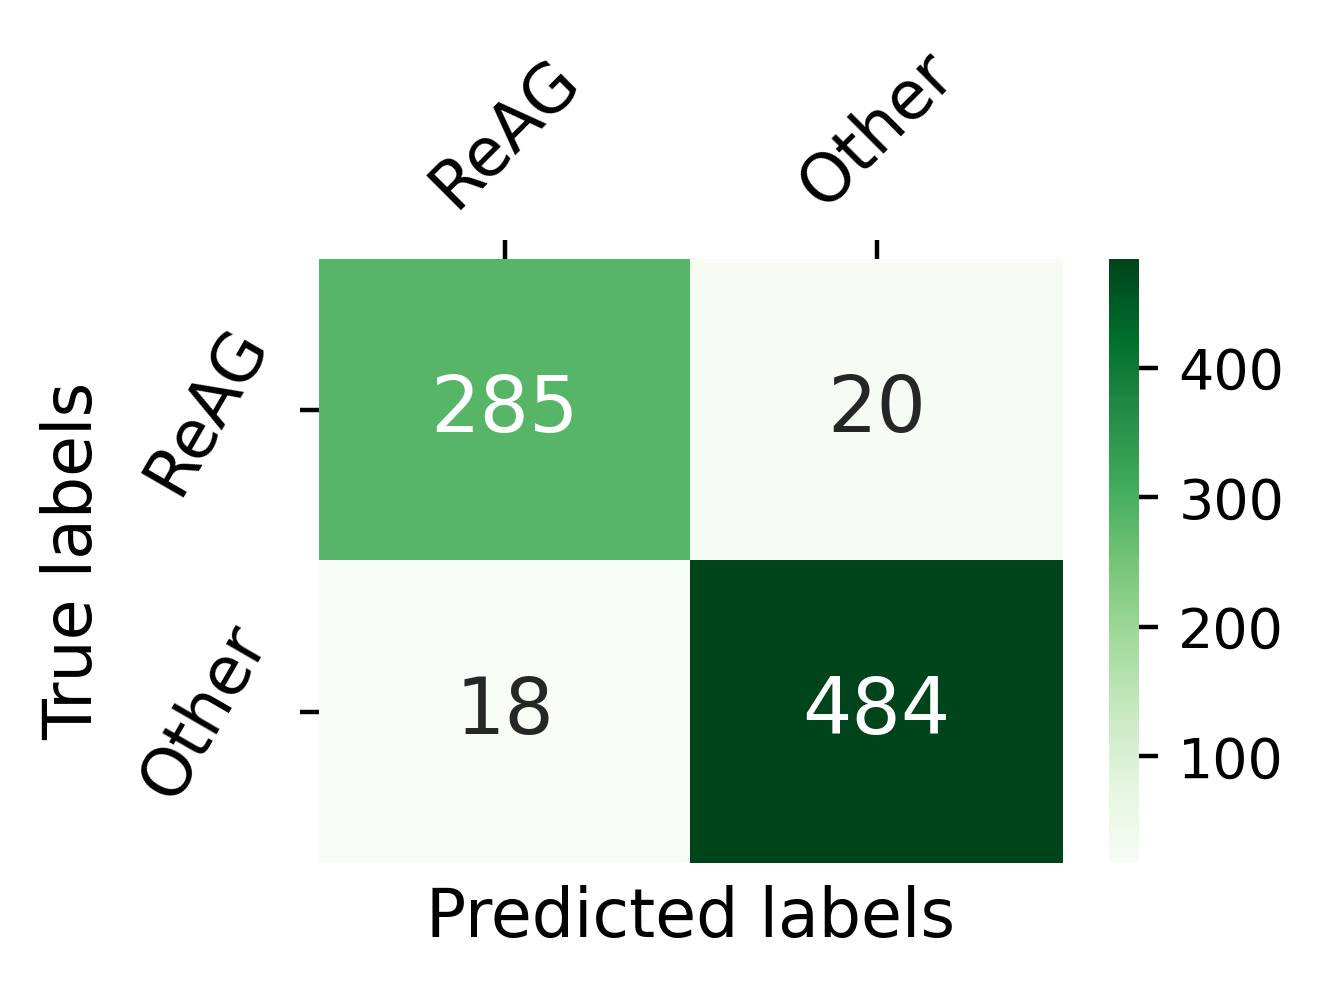
\includegraphics[width= 0.3\textwidth]{Figure/ReAG.png}}
  \subfigure[PoAG]{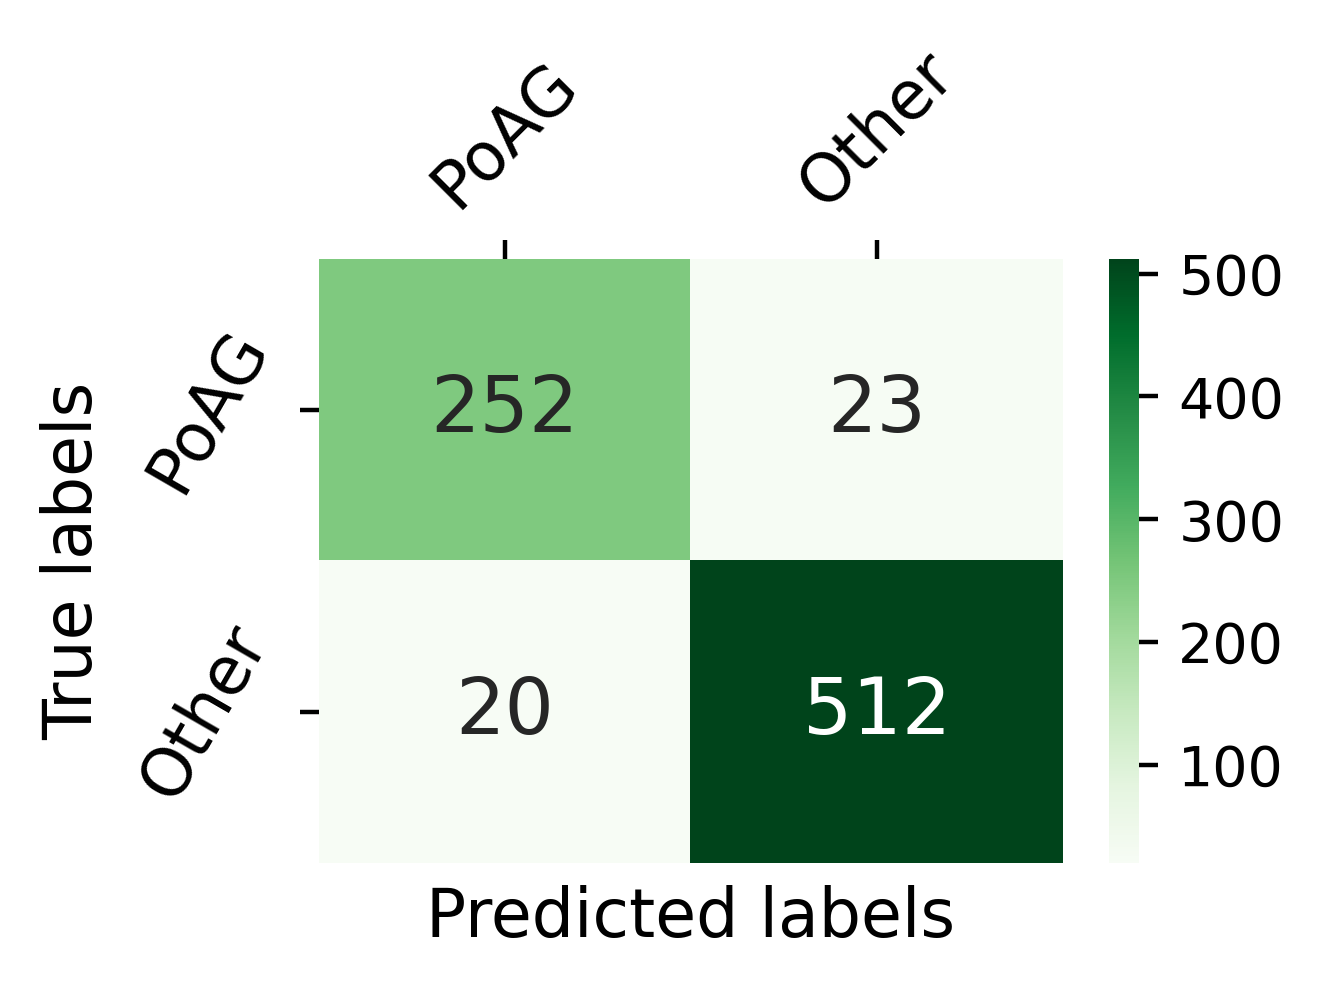
\includegraphics[width= 0.3\textwidth]{Figure/PoAG.png}}\quad
  \subfigure[VeAG]{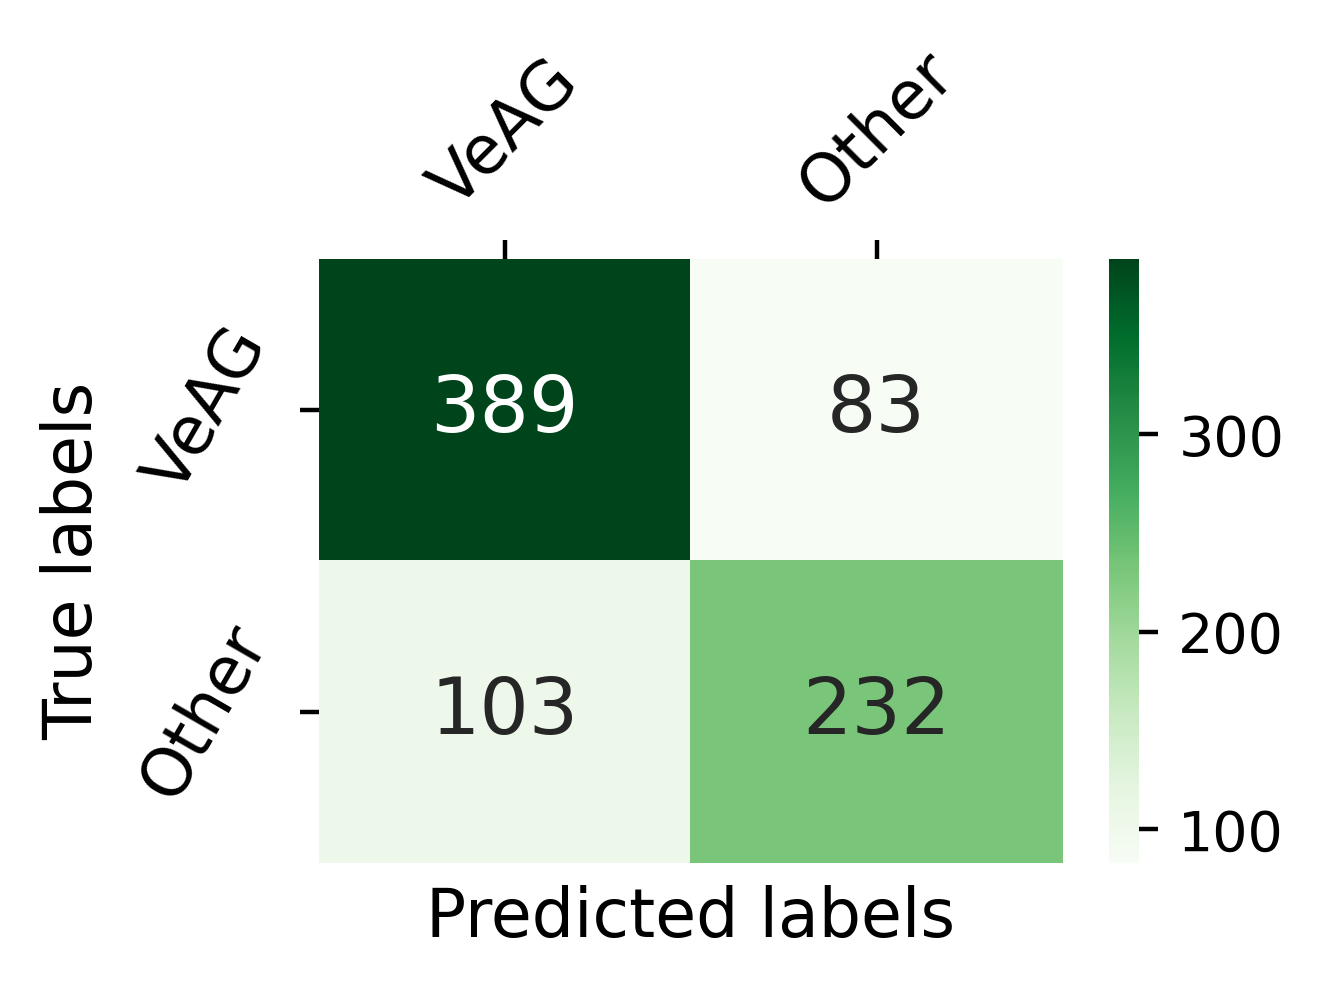
\includegraphics[width= 0.3\textwidth]{Figure/VeAG.png}}
  \subfigure[GeAG]{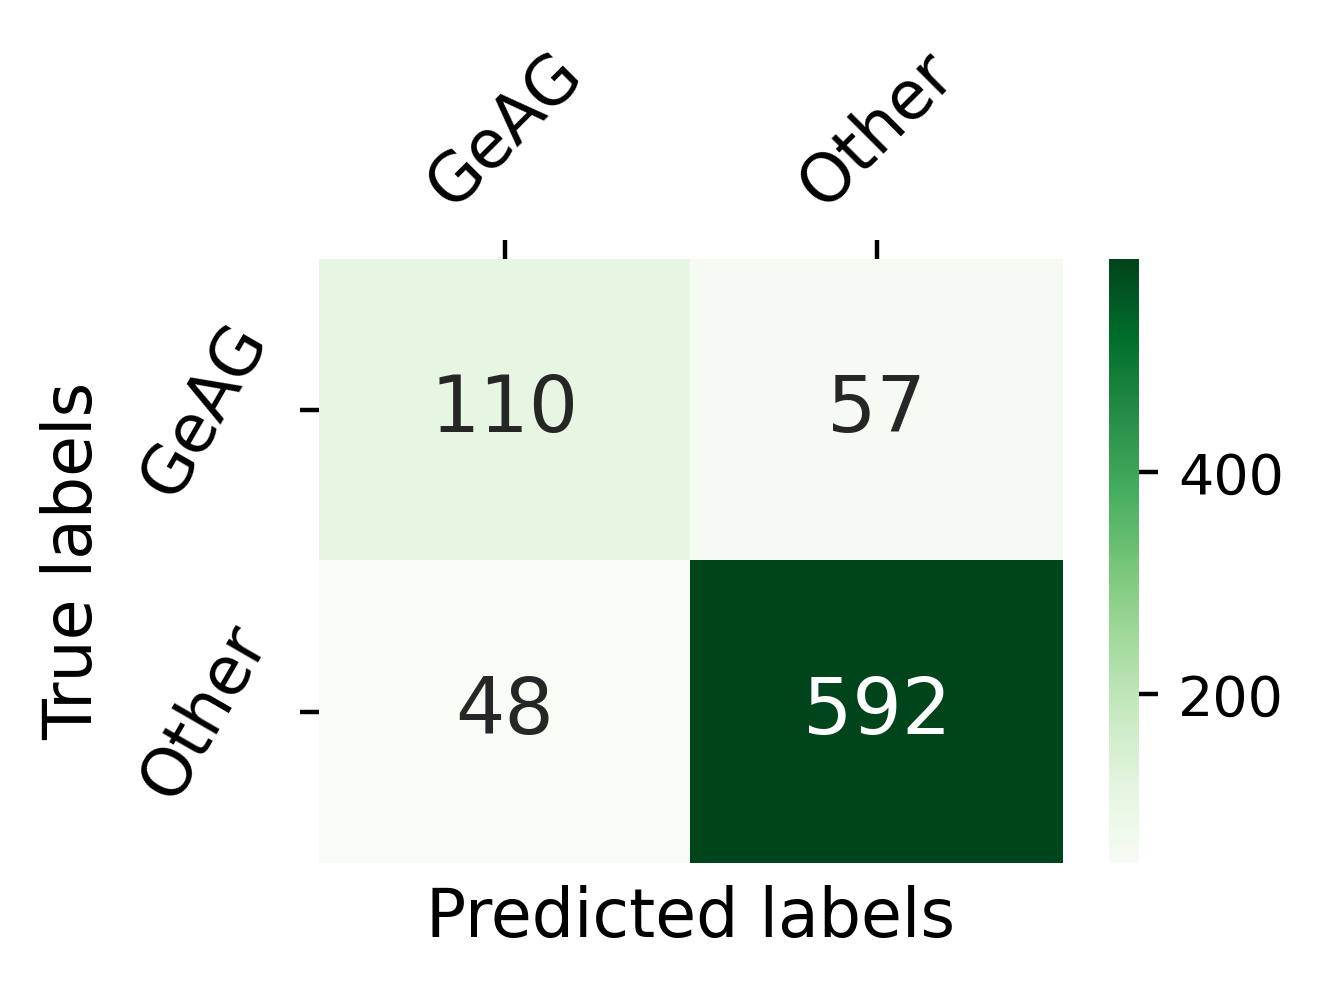
\includegraphics[width= 0.3\textwidth]{Figure/GeAG.png}}
  \subfigure[RaAG]{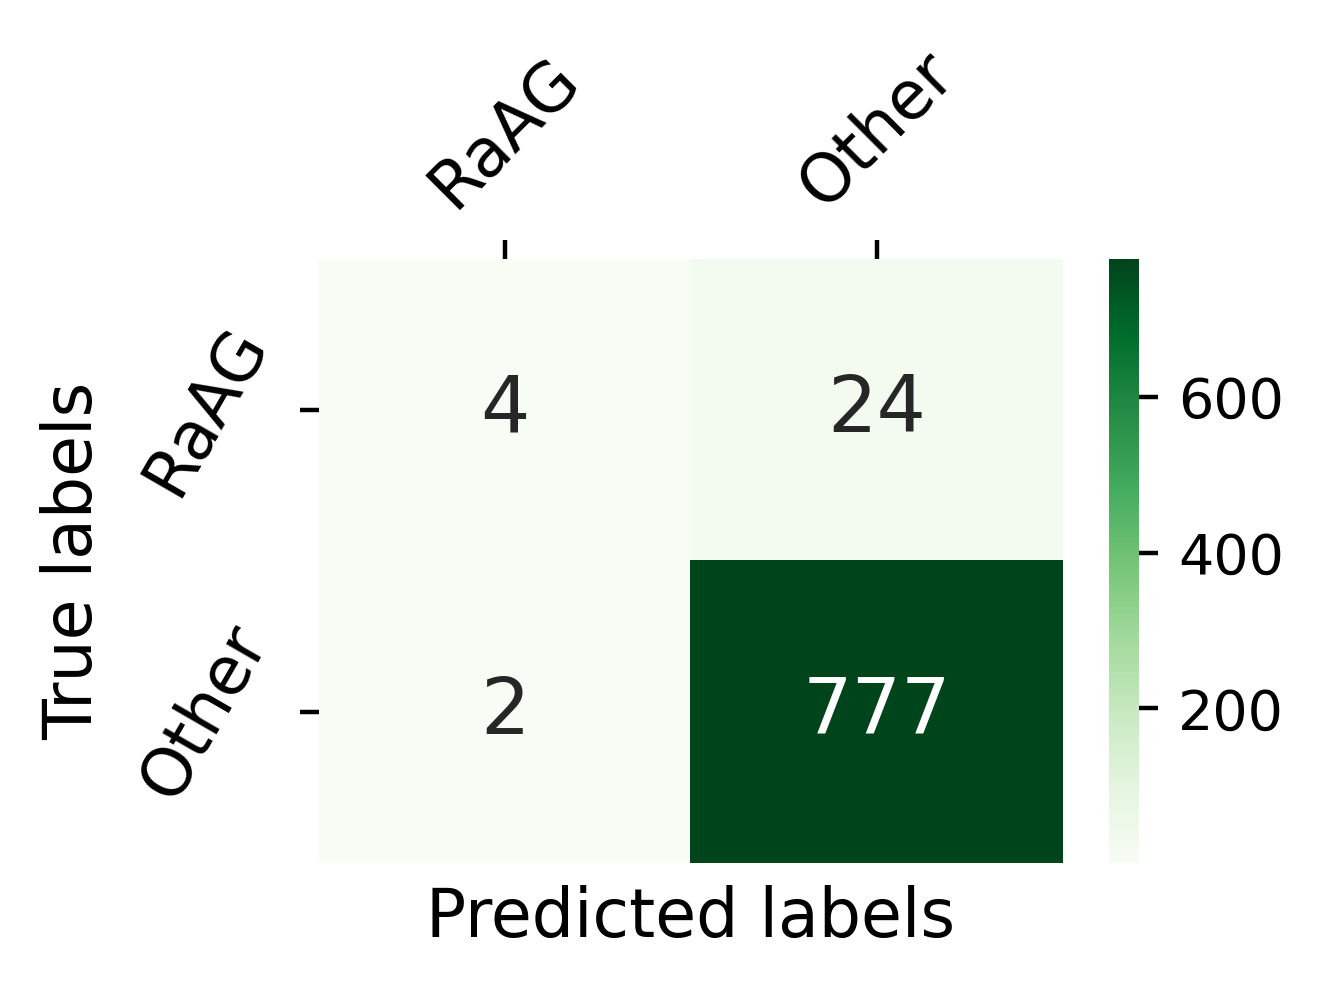
\includegraphics[width= 0.3\textwidth]{Figure/RaAG.png}}
 \caption{Confusion matrices of each category for Bangla-BERT model} 
 \label{confusion}
\end{figure*}

\subsubsection{Error Analysis}
The results confirmed that Bangla-BERT is the best performing model in both coarse-grained and fine-grained classification tasks (Table \ref{cg}, \ref{fg}). We perform a thorough error analysis to know the model mistakes across different classes.

\paragraph{Quantitative analysis:} Figure \ref{confusion} shows the confusion matrices for the Bangla-BERT model. Figure \ref{confusion} (a) depicts that with coarse-grained classification, the model incorrectly identified 73 (out of 807) and 56 (out 758) instances as NoAG and AG texts, respectively. The confusion matrices for fine-grained classes are shown in Figure \ref{confusion} (b)-(f). It is noticed that in ReAG and PoAG classes model misclassified 20 (out of 305) and 23 instances (out of 275), respectively. The model yields the most incorrect predictions (24 out of 28) with RaAG class. The reason might be that the model did not get enough samples for learning and thus failed to discern the correct class in the testing phase. Meanwhile, in the case of VeAG, the model gets confused and misclassifies other classes instance (103 out of 232) as VeAG. The appearance of outrageous words in other fine-grained aggressive classes may be the reason for this confusion. Table \ref{ea} presents the false-negative rate (FNR) of the fine-grained categories. We noticed that the FNR is very high with GeAG (0.34) class while ReAG (0.065) and PoAG (0.08) classes FNR is deficient.
     

\begin{table}[h!]

\begin{center}
%\begin{tabular}{L{1.3cm}C{1cm}C{1cm}C{1cm}C{1cm}}
\begin{tabular}{lc}
\hline
 \textbf{}  & \textbf{False negative Rate} \\
 \hline 
 ReAG  & 20/305 (0.065)  \\
 PoAG & 23/275 (0.08) \\
 VeAG & 83/472 (0.17) \\
 GeAG & 57/167 (0.34) \\
 RaAG & 4/28 (0.14) \\
 \hline
\end{tabular}
\caption{Error analysis for each fine-grained category}
\label{ea}
\end{center}
\end{table}

\paragraph{Qualitative Analysis:} Figure \ref{miss-exam} shows some correctly and misclassified sample texts from fine-grained classification tasks. The output predictions are obtained from the Bangla-BERT model. It is observed that the first two samples are correctly classified into different fine-grained aggression classes. However, in the third example, the model was only able to identify the text as \textbf{ReAG} and incorrectly predicted it as VeAG. Similarly, in the case of the last example model, it was not even able to classify it as RaAG. These examples illustrate the underlying difficulties of the multilabel classification problem. From the analysis, we found that the texts implicitly express aggression, which makes it arduous for the model to determine the multiple classes simultaneously.
Moreover, some words have extensively appeared in the fine-grained classes. Perhaps, these words confuse the model to distinguish the classes and thus makes the task more difficult. Adding more training samples across all the classes might eradicate the problem to some extent.  
      

\begin{figure*}[t!]
\centering
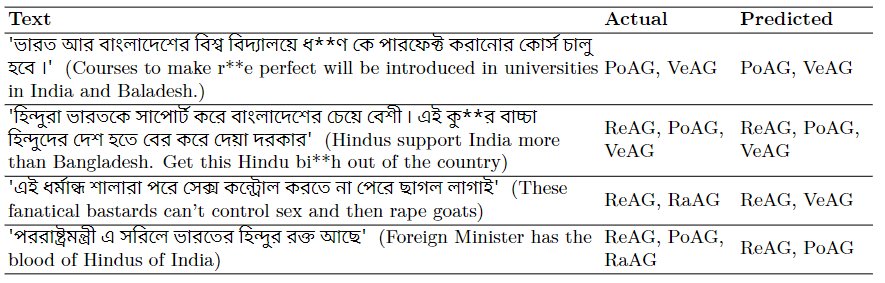
\includegraphics[width = 0.9\textwidth]{Figure/qa.PNG}
\caption{Some correctly and incorrectly classified samples by the Bangla-BERT model}
\label{miss-exam}
\end{figure*}

\section{Conclusion}
This paper presented a multilabel aggression identification system for Bengali. To accomplish the purpose, this work introduced \textit{M-BAD}, a multilabel benchmark dataset consisting of 15650 texts. A two-level hierarchical annotation schema has been followed to develop the corpus. Among the levels, Level-1 is concerned with either aggressive or not aggressive, whereas Level-2 is concerned with the targets (religious, political, verbal, gender, racial) of the aggressive texts in a multilabel scenario. Several traditional and state of the art computational models have been investigated for benchmark evaluation. The results exhibit that the Bangla-BERT model obtained the highest weighted $f_1$-score of 0.83 for the multilabel classification. The error analysis revealed that it is challenging to identify the multiple targets of aggressive text as words are frequently overlapped across different classes. In future, we aim to mitigate this issue by exploring multitask learning and domain adaption approaches. Moreover, future work considers including more data samples with a significant period to minimize the bias towards a limited set of events.      


\section*{Acknowledgements} This work supported by the ICT Innovation Fund, ICT Division, Ministry of Posts, Telecommunications and Information Technology, Bangladesh.





% Entries for the entire Anthology, followed by custom entries
\bibliography{anthology,custom}
\bibliographystyle{acl_natbib}


\appendix
\counterwithin{figure}{section}
\counterwithin{table}{section}


\section*{Appendix}
\section{Data Sources}
\label{source}
Data samples were collected from public post/comment threads of Facebook and YouTube. We did not store the profile information of any users. The data collection procedure is consistent with the copyright and terms of service of these organizations \footnote{https://www.facebook.com/help/1020633957973118, https://www.youtube.com/static?template=terms}. Potential texts were culled from more than 200 Bengali YouTube channels and Facebook pages. The popularity and activity status of a few data sources are presented in table \ref{data-sources}.

\begin{table*}[t!]
\small
\begin{center}

\begin{tabular}{L{3cm}C{1.2cm}C{2.5cm}C{3cm}C{2cm}C{2cm}}
\toprule
 \textbf{Page/channel name}& \textbf{Type} &\textbf{Affiliation}            &\textbf{ No. of followers/ subscribers}   & \textbf{Reactions per post (in avg.)} & 
 \textbf{Frequency of posting)}\\ \hline
 
 Bidyanondo & FP & Non political org. & 5M  & 10k & 10 post/day\\
  
 Prothom Alo & FP/YC & Newsgroup & 14M  & 4.5k & 180 post/day\\
 
Rafiath Mithila & FP & Artist & 3.8M  & 15k & 4 post/week\\
 
 Mizanur Azhari & YC & Religious speaker & 1.9M & 50k & 1 post/month\\
 
 Jamuna tv & FP/YC & Media  & 12.9M & 3.7k & 80 post/day\\
 
 %Asif Mohiuddin & FP & Public figure & 120k & 1k & 5 post/week\\
 
 Awami League & FP/YC & Political org. & 890k & 4.6k & 15 post/day\\
 
 Abu Toha Adnan & FP & Religious speaker & 2M & 18k & 10 post/week\\
 
 Salman BrownFish & YC/FP & Musician & 3M & 15k & 7 post/month \\
 
 %Pinaki Bhattacharya & FP & Author & 342k & 9k & 6 post/day\\
 
 Arif Azad & FP & Author & 742k & 87k & 8 post/month\\
 
 Somoynews tv& FP/YC & Media  & 8.1M & 2K & 120 post/day \\ 
 
  Basher kella & FP & Political & 45k & 400 & 15 post/day\\
  
  Roar Bangla & FP/YC & Media & 50K & 300 & 3 post/day\\
  
  Shakib Al Hasan & FP & Public figure & 15.3M & 50k & 15 post/month\\ 
 
\bottomrule
\end{tabular}
\caption{Activity and popularity statistics of a few sources from where data were gathered. FP indicates a Facebook page, and YC denotes a YouTube channel. Reactions are counted in terms of likes, comments and shares.}
\label{data-sources}
\end{center}
\end{table*}

\section{Annotator Demographics}
\label{anno-demo}
Past studies \citep{suhr-etal-2021-crowdsourcing, zhou-etal-2021-challenges} on benchmark dataset creation have emphasized knowing about the demographic, geographic, research and other related information of the annotators. Since aggression is a very subjective phenomenon, annotators perspective and experience play a crucial role in developing the dataset. Six students and an expert were involved in our dataset construction process. Annotators demographic information, research experience, the field of research, and personal experience of viewing online aggression are summarized in table \ref{ano-info}.

\begin{table*}[ht!]
\small
\begin{center}

\begin{tabular}{lccccccC{2cm}}
\toprule
 & \textbf{AN-1} &\textbf{AN-2} &\textbf{AN-3}   &\textbf{AN-4}&\textbf{AN-5}&\textbf{AN-6} & \textbf{Expert} \\ \hline
 Research-status  & Undergrad & RA  & Undergrad   & Graduate  & RA & Graduate & Professor \\
 Research area  &  NLP  & NLP & NLP  & NLP & NLP & NLP  & NLP, Social computig, HCI\\
 Experience (years) & 1 & 1 & 0.5 & 2.5 &1.5 & 3 & 21 \\
 Prior annotation experience & yes   & yes & no  & yes  & yes & yes & yes \\
\midrule
Gender  &  Male  & Male  & Female   & Female  & Male & Male & Male\\
Age  &  22  & 23 & 22 & 25 & 23 & 26 & 47 \\
Religion  & Islam & Hindu  & Hindu   & Islam & Islam & Islam &Islam  \\
\midrule
Viewed online aggression & yes   & yes & yes  & yes  & yes & yes & yes \\
Targeted by online aggression & yes   & no & no  & yes  & no & yes & yes \\
\bottomrule
\end{tabular}
\caption{Summary of annotators information.}
\label{ano-info}
\end{center}
\end{table*}

Some key characteristics of the annotators' pool are, (i) native Bengali speakers, (ii) have prior experience of annotation, (iii) not an active member of any political parties, (iv) not hold extreme view against religion, (v) viewed online aggression. Before requiting, the annotators' necessary ethical approval was taken, and they are substantially paid according to university regulations. 

\section{Data Samples}
\label{sample}
The authors would like to state that the examples referred to in the figure \ref{examp} presented as they were accumulated from the source. Authors do not use these examples to hurt individuals or promote aggressive language usage. The goal of this work is to mitigate the propagation of such language.
\begin{figure*}[t!]
\centering
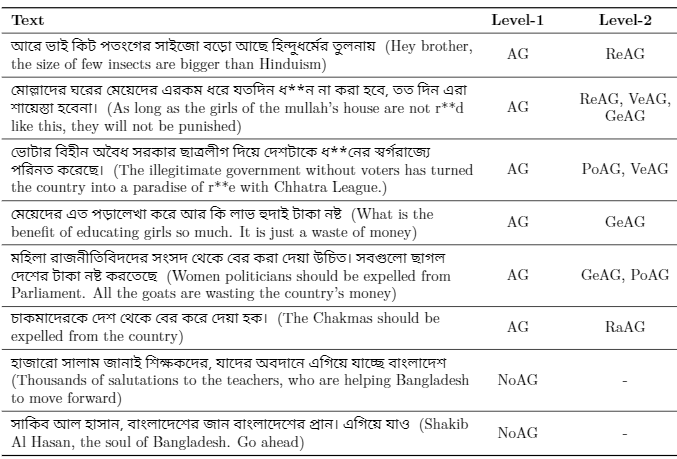
\includegraphics[width =0.95\textwidth]{Figure/example.PNG}
\caption{Few samples of M-BAD}
\label{examp}
\end{figure*}


\end{document}
